\section{The selection integral decides the answer}
\label{sec:selection}

Three results in this paper are, at bottom, statements about the selection
integral. The first is practical: on a sparse tracer the selection Monte Carlo
must follow the catalog or the measurement is invalid
(\S\ref{sec:selection:proposal}). The second is a mechanism: the clustered
mocks' distance-scale deficit of \S\ref{sec:fraction:joint} is the incomplete
cancellation of two spurious levers sprung by a single inconsistency between
the detection rule and the likelihood's distance-space selection
(\S\ref{sec:selection:tilt}). The third is the one genuinely multitracer
effect of the three: the sparse tracer, precisely because it is sparse,
anchors the distance scale against that inconsistency, and the growth of the
deficit with \fagn\ is the loss of an accidental cancellation, not a new
pathology (\S\ref{sec:selection:anchor}).

\subsection{A sparse tracer needs its own proposal}
\label{sec:selection:proposal}

On the matched two-tracer mock, with \DeepNobs\ events at a planted
$\fagn = \DeepFTruth$, injections drawn from the source population give an
effective sample size for the selection integral that \emph{falls} as the
mixture leans on the sparse tracer: \NeffPopNought\ at
$\fagn = \NeffFNought$, then
\NeffPopThree, \NeffPopSeven\ and \NeffPopUnity\ at
$\fagn = \NeffFThree$, \NeffFSeven\ and \NeffFUnity, against a floor of
\NeffFloor\ --- a decay by a factor of
\NeffPopDecay\ across the grid, with three of the four points below the floor
(Figure~\ref{fig:lane}a). Adding a branch that places \InjWtgt\ of the proposal
at catalogued AGN reverses the trend: \NeffTgtNought, \NeffTgtThree,
\NeffTgtSeven\ and \NeffTgtUnity, a \emph{rise} by a factor of
\NeffTgtRise. The honest cost sits at $\fagn = \NeffFNought$, where moving proposal weight
off the dense tracer gives up \NeffTgtCostAtZero\% of its effective sample size
and still clears the floor by a factor of \NeffTgtMarginAtZero.

What that buys is not precision but validity. At the reduced sample of
\DeepSmallNobs\ events, where the untargeted campaign is still usable at all,
only \DeepFPopAdm\ of \DeepFPopCells\ grid cells are admissible, the admissible
range ends at $\fagn = \DeepFPopAdmHi$, and the posterior peaks against that very
edge: it reports $\fagn = \DeepFPopMed$ with a 68\% interval of
$[\DeepFPopLo, \DeepFPopHi]$, which contains the planted value and means nothing,
because the interval is set by where the selection estimate stopped being usable
(Figure~\ref{fig:lane}b). With the same events and only the injection set
changed, every cell becomes admissible and the peak moves from
$\fagn = \DeepFPopMed$ to $\DeepFSmallTgtMed$ --- about two half-widths, so
the campaign changes the answer and not merely its reliability. The
measurement itself is made on the repaired-generator events of
\S\ref{sec:budget:oracle}, whose detected set, catalogs and injection
campaigns are identical to the exhibit above and whose posterior construction
is what the repair fixed: the targeted campaign gives
$\fagn = \DeepFixFSmallMed$ $[\DeepFixFSmallLo, \DeepFixFSmallHi]$ at
\DeepSmallNobs\ events, and at the full sample --- which the targeted
campaign is what makes reachable --- $\fagn = \DeepFixFTgtMed$ with
$[\DeepFixFTgtLo, \DeepFixFTgtHi]$: \DeepFixFTgtOffAbs\ below the planted
value on a \DeepFixFTgtHw\ half-width, \DeepFixFTgtSig$\sigma$, with the
planted value inside the 90\% interval.

\begin{figure*}
\centering
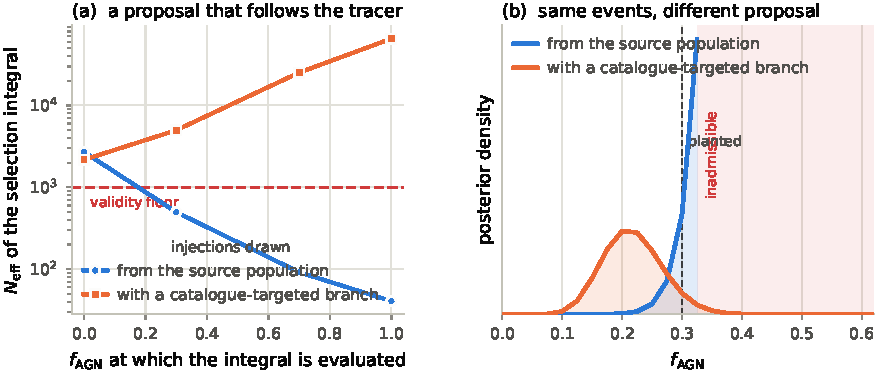
\includegraphics[width=\textwidth]{figures/fig_selection_lane.pdf}
\caption{Why a sparse tracer needs its own selection proposal, on the matched
two-tracer mock. \emph{(a)} effective sample size of the catalog-conditioned
selection integral against the fraction at which it is evaluated, at the full
sample of \DeepNobs\ events, for injections drawn from the source population and
for a proposal that places \InjWtgt\ of its draws at catalogued AGN; the dashed
line is the reliability floor $5\,\Nobs$. \emph{(b)} the fraction's posterior
from the same \DeepFPopCells-point scan with the two campaigns, at the reduced
sample where the untargeted one is still evaluable at all; shading marks
inadmissible cells. The untargeted posterior peaks against the edge of the
admissible region, so its apparent agreement with the planted value carries no
information. The comparison holds the events fixed (the mock as first
generated); the generator repair of \S\ref{sec:budget:oracle} changes neither
the detected set nor the injections, so it leaves this campaign-versus-campaign
statement untouched.
\label{fig:lane}}
\end{figure*}

The joint plane on this mock is interpretable for the first time with the
targeted campaign: $\Hz = \DeepFixJointHzero$ $[\DeepFixJointHzeroLo,
\DeepFixJointHzeroHi]$~\kmsmpc\ and $\fagn = \DeepFixJointF \pm
\DeepFixJointFHw$ with $\rho = \DeepFixJointRho$. Of \DeepJointCells\ cells,
\DeepFixJointRej\ are inadmissible, but all of them lie at expansion rates
far from the peak: the posterior mass adjacent to the inadmissible region is
$\DeepFixJointMassAdj$, and none of the 68\% region touches it. Both
parameters land within about one half-width of the truth ---
\DeepFixJointHzeroOff~\kmsmpc\ on the expansion rate
(\DeepFixJointHzeroSig$\sigma$) and \DeepFixJointFSig$\sigma$ on the fraction
--- and with $\rho \simeq 0$ they are measured essentially independently. The
same scans on the mock as first generated had returned \Hz\
\DeepJointHzeroOffAbs~\kmsmpc\ low (\DeepJointHzeroSig$\sigma$) and the
fraction \DeepFTgtSig$\sigma$ low; the sky-width repair of
\S\ref{sec:budget:oracle}, which changes only the fidelity of the mock's
posterior construction, removes both, so the two-tracer measurement inherits
the closure of the single-tracer budget rather than merely being consistent
with it.

Two points are worth carrying forward. First, this is the second place in this
programme where the binding constraint on a field-mode multitracer measurement
was the resolution of the selection Monte Carlo rather than the
gravitational-wave data; it appears to be a structural property of conditioning
the selection integral on a sparse catalog, and any analysis that does so needs
a proposal that follows the tracer. Second, the complete-catalog limit obtained
by driving the assumed density to zero is far worse conditioned than the
incomplete model evaluated at a true density anchor: on the same mock the
anchored incomplete model reaches $\Neff = \IncCompleteNeff \times 10^3$ against
$\NeffTgtThree$ for the complete-catalog trick. The trick buys an unbiased
complete-catalog limit at a real cost in selection resolution.

\subsection{One inconsistency, two levers: the clustered mocks' deficit}
\label{sec:selection:tilt}

The distance-scale deficit of \S\ref{sec:fraction:joint} --- \Hz\ low by
\BaseJointHzeroOffAbsThree~\kmsmpc\ at $\fagn = \BaseFTruthThree$ and
\BaseJointHzeroOffAbsSeven\ at \BaseFTruthSeven, with the fraction recovered
correctly --- has a complete mechanical explanation, obtained from a
term-by-term rebuild of the likelihood that reproduces the production curves to
better than $10^{-3}$~nats and can then be evaluated with counterfactual
switches. The origin is one inconsistency: the mocks detect events by a cut on
\emph{true source redshift}, $z \le \GlassZtrunc$, while the likelihood
expresses both its selection integral and its host prior in \emph{luminosity
distance}, against catalogs whose support continues to $z = \GlassZmax$ ---
\TiltCatAboveGal\% of the galaxies and \TiltCatAboveAgn\% of the AGN lie above
the horizon no detected event can occupy. That single mismatch springs two
opposing levers.

\emph{The selection lever
(\BaseDecompShiftThree\ / \BaseDecompShiftSeven~\kmsmpc\ at the two planted
fractions).} Because the injections carry exact distances at the true
cosmology, the detected injection set fills exactly
$d_L \le \TiltDlmax$~Mpc, the distance of the horizon. Under the analysis
model at trial \Hz\ that fixed distance boundary sits at a redshift
$z^*(\Hz)$ that sweeps from \TiltZstarLo\ at $\Hz = 60$ to \TiltZstarHi\ at
75: raising \Hz\ pushes $z^*$ up the still-rising catalog $\dd N/\dd z$, so
the detectable fraction $\mu$ \emph{rises} with \Hz\
($\dd\ln\mu/\dd\Hz = \TiltSlopeMeasThree$ at truth) when for a true-redshift
cut it should be flat. Multiplied by $-\Nobs$ this is a
$-\TiltSelSlopeNatsThree$~nats per \kmsmpc\ lever. A zero-parameter analytic
model --- the catalog's redshift distribution integrated to $z^*(\Hz)$ with
the population's rate weighting --- predicts a slope of \TiltSlopeModelThree,
\TiltModelPct\% of the measured value, and re-peaking the likelihood against
it reproduces \TiltPredShiftThree\ of the \BaseDecompShiftThree\ shift. The
lever is not an artifact of injection coverage: recomputing $\mu(\Hz)$ with an
untargeted, independently seeded injection set changes the slope by
\TiltSlopeDiffPct\%. The estimator faithfully computes the model's $\mu$; the
model's $\mu$ is what is wrong for this detection rule.

\emph{The numerator lever (\TiltNumLeakThree\ / \TiltNumLeakSeven~\kmsmpc,
opposing).} Events exist only below the horizon, but the host prior does not:
the broad distance posteriors of near-horizon events map part of their mass to
$z(d_L; \Hz) > 1$, where the catalogs still offer (spurious, for detected
events) support. The mean posterior mass beyond the horizon is
\TiltLeakTruthThree\% at truth and \TiltLeakHighThree\% at $\Hz = 75$ (at
$\fagn = \BaseFTruthThree$; \TiltLeakTruthSeven\% and \TiltLeakHighSeven\% at
\BaseFTruthSeven), so raising \Hz\ maps more posterior mass higher up the
rising $\dd N/\dd z$ and the per-event term grows with \Hz. Masking the host
prior above the horizon removes essentially the whole numerator offset
(\BaseDecompNumOffThree\ $\rightarrow$ \TiltRepairOffThree). This also
explains the catalog-edge lever of \S\ref{sec:fraction:joint}: truncating the
catalogs at $z \le 1$ removed the numerator's upward pull while leaving the
selection slope uncompensated, which is why the data-free relocation of a
catalog boundary moved \Hz\ by \BaseEdgeShiftThree~\kmsmpc.

The two levers account for the deficit in full. Repairing both at once --- a
host prior truncated at the detection horizon together with the
$\Hz$-independent selection normalisation the true-redshift cut actually
implies --- returns the peak to \TiltRepairOffThree~$\pm$~\TiltRepairSigThree~\kmsmpc\
of the truth at $\fagn = \BaseFTruthThree$ and \TiltRepairOffSeven\ at
\BaseFTruthSeven\ (Figure~\ref{fig:tilt}); repairing either alone makes the
bias worse, because the levers are opposed. The delta-method Monte Carlo bias
of the per-event estimates contributes at most \TiltMcBiasMax~\kmsmpc. For
real data the transferable statement is about consistency rather than about
this mock: the selection function must be expressed in the variable that
actually decided detection, and a host prior with support well beyond the
detected population's horizon hands the numerator spurious \Hz\ information of
order the posterior-mass leak whenever the distance posteriors are broad.

\begin{figure*}
\centering
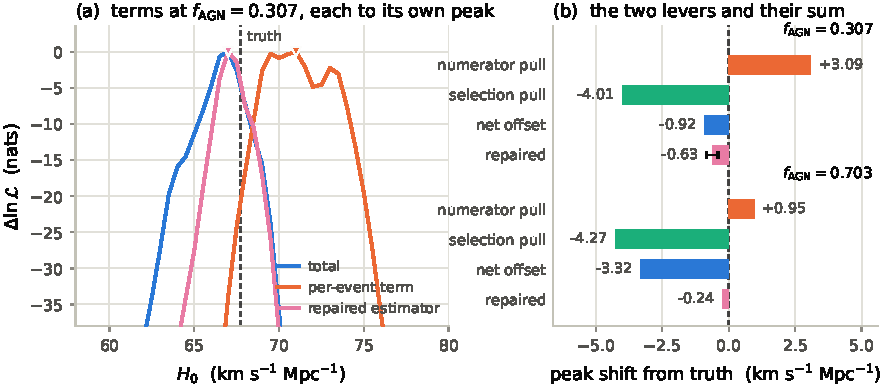
\includegraphics[width=\textwidth]{figures/fig_tilt_decomposition.pdf}
\caption{The clustered mocks' distance-scale deficit decomposed, at fixed
planted fractions. \emph{(a)} log-likelihood terms against \Hz\ at
$\fagn = \BaseFTruthThree$, each normalised to its own peak: the per-event
term peaks \BaseDecompNumOffThree~\kmsmpc\ high, and the selection term ---
a near-linear tilt of $\sim\TiltSelSlopeNatsThree$~nats per \kmsmpc\ with no
interior peak, visible here as the displacement between the per-event term
and the total --- pulls the total down by \BaseDecompShiftThree. The repaired
estimator --- host prior truncated at the detection horizon, selection
normalisation matched to the true-redshift cut --- peaks at the truth. \emph{(b)} the same budget at both
planted fractions: the selection lever is nearly independent of the fraction
while the numerator pull collapses as the mixture weight moves onto the
sparse tracer (\S\ref{sec:selection:anchor}), so the net deficit grows.
\label{fig:tilt}}
\end{figure*}

\subsection{The sparse tracer anchors the distance scale}
\label{sec:selection:anchor}

Why does the deficit grow with \fagn\ when both levers are set by the same
catalogs? Not through the redshift distributions --- the two tracers'
$\dd N/\dd z$ shapes are identical to within a fraction of a per cent
(\TiltCatAboveGal\% versus \TiltCatAboveAgn\% of objects above the horizon)
--- and indeed the selection lever barely moves
(\BaseDecompShiftThree\ $\rightarrow$ \BaseDecompShiftSeven). What changes is
the numerator, and the reason is sparseness. With \GlassNagn\ AGN spread over
\GlassNpix\ pixels, \GlassAgnEmptyPix\% of the sky holds none, and within an
event's localisation the AGN branch of the mixture is a handful of
near-delta-function redshift kernels of width $\sigma_z = \GlassDzScale(1+z)$:
effectively a noisy counterpart prior. It pins the distance scale. The
per-event term of AGN-hosted events peaks at
\TiltNumAgnhostThree~\kmsmpc\ (\TiltNumAgnhostOffThree\ from truth), while
that of galaxy-hosted events --- whose smooth, deep prior is maximally exposed
to the above-horizon support --- peaks at \TiltNumGalhostThree\
(\TiltNumGalhostOffThree). As the planted fraction rises from
\BaseFTruthThree\ to \BaseFTruthSeven\ the mean posterior weight on the
anchored branch grows from \TiltAgnShareThree\ to \TiltAgnShareSeven, the
numerator's spurious pull collapses from \BaseDecompNumOffThree\ to
\BaseDecompNumOffSeven~\kmsmpc\ and its curvature nearly doubles
(\TiltCurvThree\ $\rightarrow$ \TiltCurvSeven\ nats per (\kmsmpc)$^2$), while
the selection lever stays put: the net deficit deepens from
\BaseJointHzeroOffThree\ to \BaseJointHzeroOffSeven. The value at
$\fagn = \BaseFTruthThree$ is accurate by cancellation, not by correctness.
The offset at the higher fraction is robust to the selection realisation:
three independent injection sets give \TiltInjSpreadMean~$\pm$~\TiltInjSpreadSd~\kmsmpc.

Read as multitracer physics rather than as a bug report, this is a positive
result. A sparse, strongly clustered tracer contributes exactly what a
statistical analysis lacks: near-counterpart redshift anchors that make the
per-event term robust against mis-modelled prior support. The anchoring is
invisible in a correct analysis --- the repaired estimator recovers the truth
at both fractions --- but it means that the population most often analysed,
dense smooth catalogs at $\fagn = 0$, is also the configuration most exposed
to selection--prior inconsistencies of this kind.
